%!TEX root = ../../main.tex


A primeira fase do treinamento dos modelos foi conduzida utilizando a arquitetura LeNet. Nesta fase, foi realizada uma busca em \emph{grid} por todos os hiperparâmetros previamente definidos, conforme Seção \ref{sec:modelos}, gerando um total de $36$ modelos a serem treinados e testados. Para estes modelos, excluindo aqueles que se tornaram degenerados, utilizou-se a métrica \emph{F-score} como referência para um melhor desempenho

Os quatro melhores modelos baseados na arquitetura LeNet para este problema encontram-se dispostos na Tabela \ref{tab:lenet}, juntamente com os hiperparâmetros utilizados pelos mesmos. Apenas para referência posterior, considerou-se uma rotulação das melhores redes identificadas.

\begin{table}[h]
\centering
\caption{Detalhamento dos melhores resultados obtidos com a arquitetura LeNet, organizados de forma decrescente considerando o valor de acurácia.}
\label{tab:lenet}
\begin{tabular}{cccccc}
\toprule
\textbf{Identificação} & \textbf{Otimizador} & \textbf{\emph{Patience}}  & \textbf{Função de Ativação} & \textbf{Acurácia} & \textbf{F-Score} \\
\midrule
LeNet A & RMSprop & 5 & ReLU & $0.9865$ & $0.9755$ \\
LeNet B & RMSprop & 15 & ReLU & $0.9858$ & $0.9740$\\
LeNet C & SGD & 5 & ELU & $0.9787$ & $0.9619$ \\
LeNet D & RMSprop & 10 & SELU & $0.9707$ & $0.9483$ \\
\bottomrule
\end{tabular}
\end{table}


Os gráficos da Figura \ref{fig:treinamento-lenet} denotam o histórico da perda (\emph{loss}) e acurácia para o conjunto de treinamento e validação destas redes. Nota-se que nenhuma delas chegou ao limite máximo de épocas possíveis, interrompendo o aprendizado por meio de \emph{early stopping}.

\begin{figure}[h!]
	\centering
	\caption{Histórico de \emph{loss} e acurácia durante o treinamento dos melhores modelos obtidos com a arquitetura LeNet.}
	\subfloat[\emph{Loss} durante treinamento da rede LeNet A.\label{subfig:lenet-a-loss}]{%
	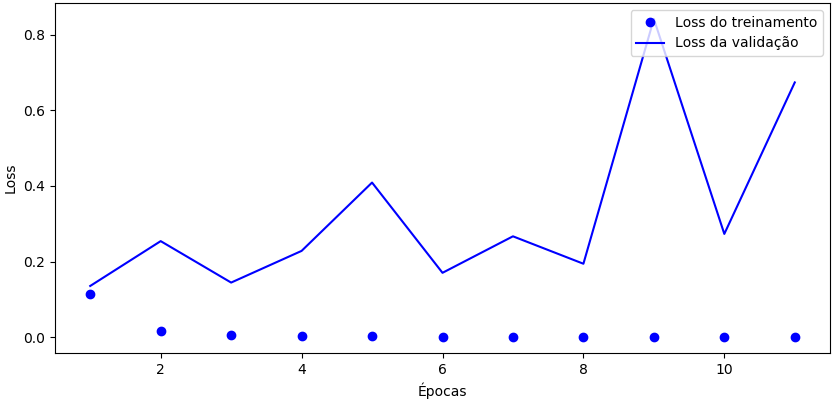
\includegraphics[width=0.45\textwidth]{imgs/lenet-a-loss}
	}
	\subfloat[Acurácia durante treinamento da rede LeNet A.\label{subfig:lenet-a-acc}]{%
	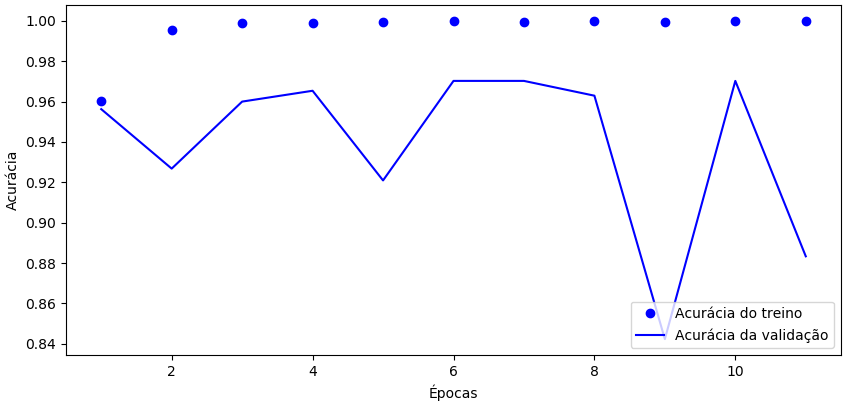
\includegraphics[width=0.45\textwidth]{imgs/lenet-a-acc}
	}
	\hfill
	\subfloat[\emph{Loss} durante treinamento da rede LeNet B.\label{subfig:lenet-b-loss}]{%
	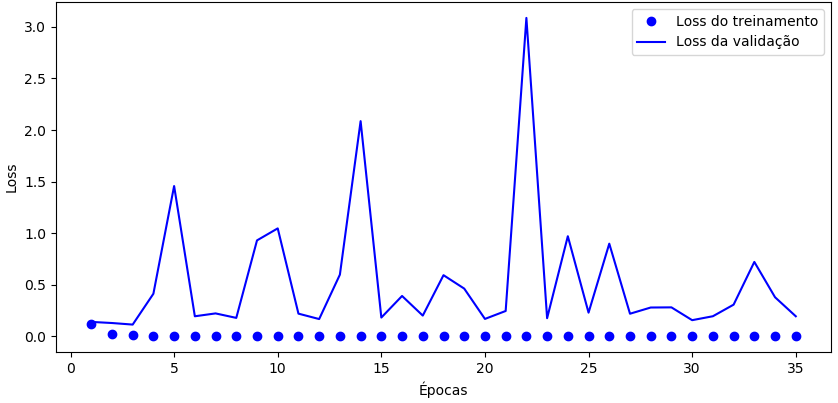
\includegraphics[width=0.45\textwidth]{imgs/lenet-b-loss}
	}
	\subfloat[Acurácia durante treinamento da rede LeNet B.\label{subfig:lenet-b-acc}]{%
	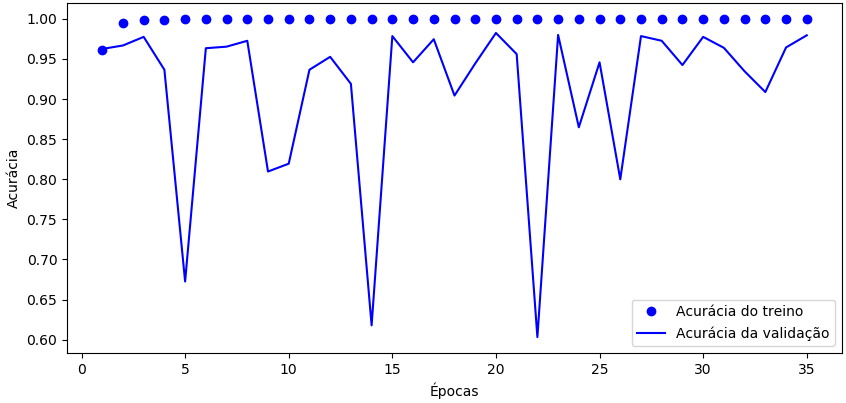
\includegraphics[width=0.45\textwidth]{imgs/lenet-b-acc}
	}
	\hfill
	\subfloat[\emph{Loss} durante treinamento da rede LeNet C.\label{subfig:lenet-c-loss}]{%
	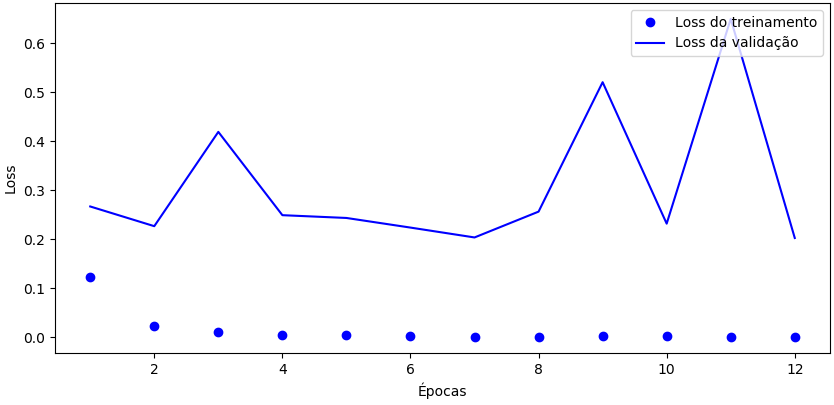
\includegraphics[width=0.45\textwidth]{imgs/lenet-c-loss}
	}
	\subfloat[Acurácia durante treinamento da rede LeNet C.\label{subfig:lenet-c-acc}]{%
	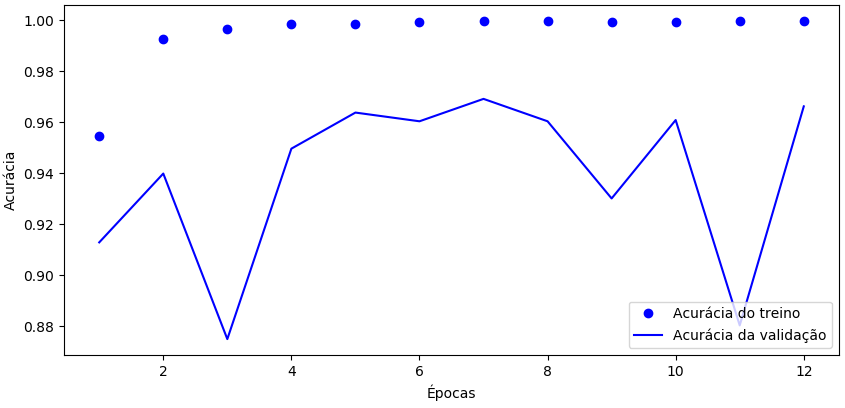
\includegraphics[width=0.45\textwidth]{imgs/lenet-c-acc}
	}
	\hfill
	\subfloat[\emph{Loss} durante treinamento da rede LeNet D.\label{subfig:lenet-d-loss}]{%
	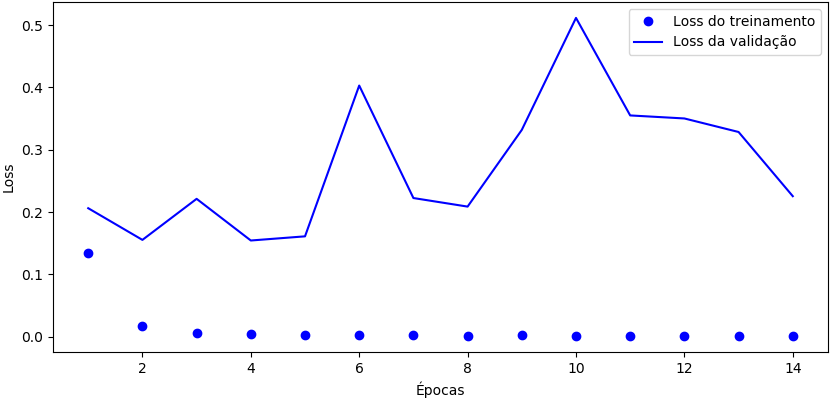
\includegraphics[width=0.45\textwidth]{imgs/lenet-d-loss}
	}
	\subfloat[Acurácia durante treinamento da rede LeNet D.\label{subfig:lenet-d-acc}]{%
	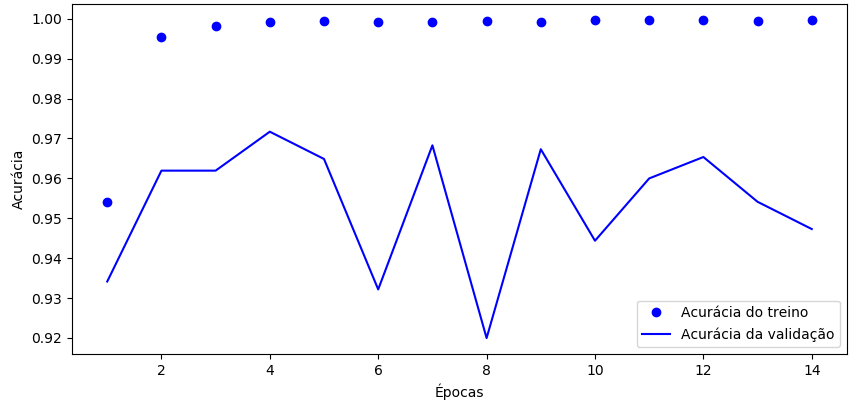
\includegraphics[width=0.45\textwidth]{imgs/lenet-d-acc}
	}
	\label{fig:treinamento-lenet}
\end{figure}

Examinando mais atentamente o desempenho destas redes no conjunto de testes, tem-se, então, as matrizes de confusão mostradas na Figura \ref{fig:matrizes-lenet}. Nestas matrizes, a soma das linhas representam a quantidade de assinaturas previstas para cada classe pelo modelo em questão, enquanto a soma das colunas denotam a quantidade de assinaturas existentes em cada classe.

\begin{figure}[h]
	\centering
	\caption{Matrizes de confusão dos melhores modelos obtidos com a arquitetura LeNet.}\label{fig:matrizes-lenet}
	\subfloat[LeNet A\label{subfig:matriz-lenet-a}]{%
	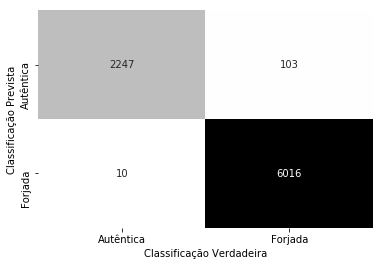
\includegraphics[width=0.5\textwidth]{imgs/matriz-lenet-a}
	}
	\subfloat[LeNet B\label{subfig:matriz-lenet-b}]{%
	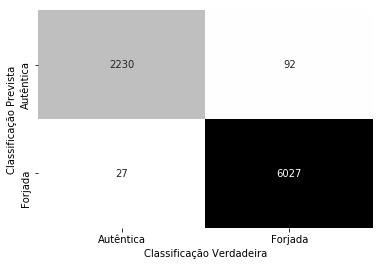
\includegraphics[width=0.5\textwidth]{imgs/matriz-lenet-b}
	}
	\hfill
	\subfloat[LeNet C\label{subfig:matriz-lenet-c}]{%
	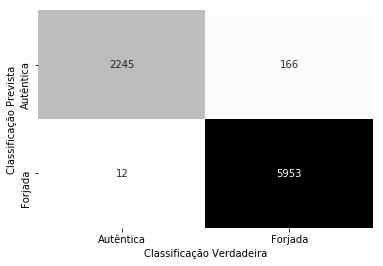
\includegraphics[width=0.5\textwidth]{imgs/matriz-lenet-c}
	}
	\subfloat[LeNet D\label{subfig:matriz-lenet-d}]{%
	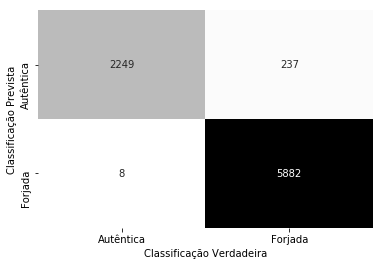
\includegraphics[width=0.5\textwidth]{imgs/matriz-lenet-d}
	}
\end{figure}

%%%% ARGUMENTAÇÃO

Para esta arquitetura, é possível visualizar que dentre os melhores modelos houve uma prevalecência do otimizador RMSProp como sendo o mais adequado. O número de épocas para aprendizado das características foi, em geral, baixo. Isso acontece porque os exemplos não possuem informação de cor e as características de interesse para identificação do autor possivelmente são de fácil extração, o que não demanda múltiplas épocas até sua obtenção.

A partir das matrizes de confusão, percebeu-se que a  maioria dos modelos tendeu a um baixo número de falsos negativo, ou seja, os exemplos autênticos fornecidos foram suficientes para identificar assinaturas originais, independentemente das variações cometidas por este autor. Porém, verifica-se uma presença proporcionalmente maior de falsos positivos, ou seja,  há assinaturas forjadas que se passam por assinaturas autênticas segundo os classificadores construídos. Isto se deve, potencialmente, à boa capacidade de certos forjadores \emph{over-the-shoulder} em fazer reproduções verossímeis não capturadas pelas CNNs propostas. Apesar disso, nota-se a diagonal principal bastante densa, sugerindo uma boa adequação dos modelos para a tarefa considerada ainda que diante de falsificações nunca antes vistas.
